\section{Diagrams}

\subsection{UML (Unified Modeling Language)}
UML (Unified Modeling Language) is a standardized modeling language used to visualize, design, and document the structure and behavior of software systems. It provides a graphical representation of the system architecture, relationships, and interactions between components.

\vspace{0.5cm}
\begin{center}
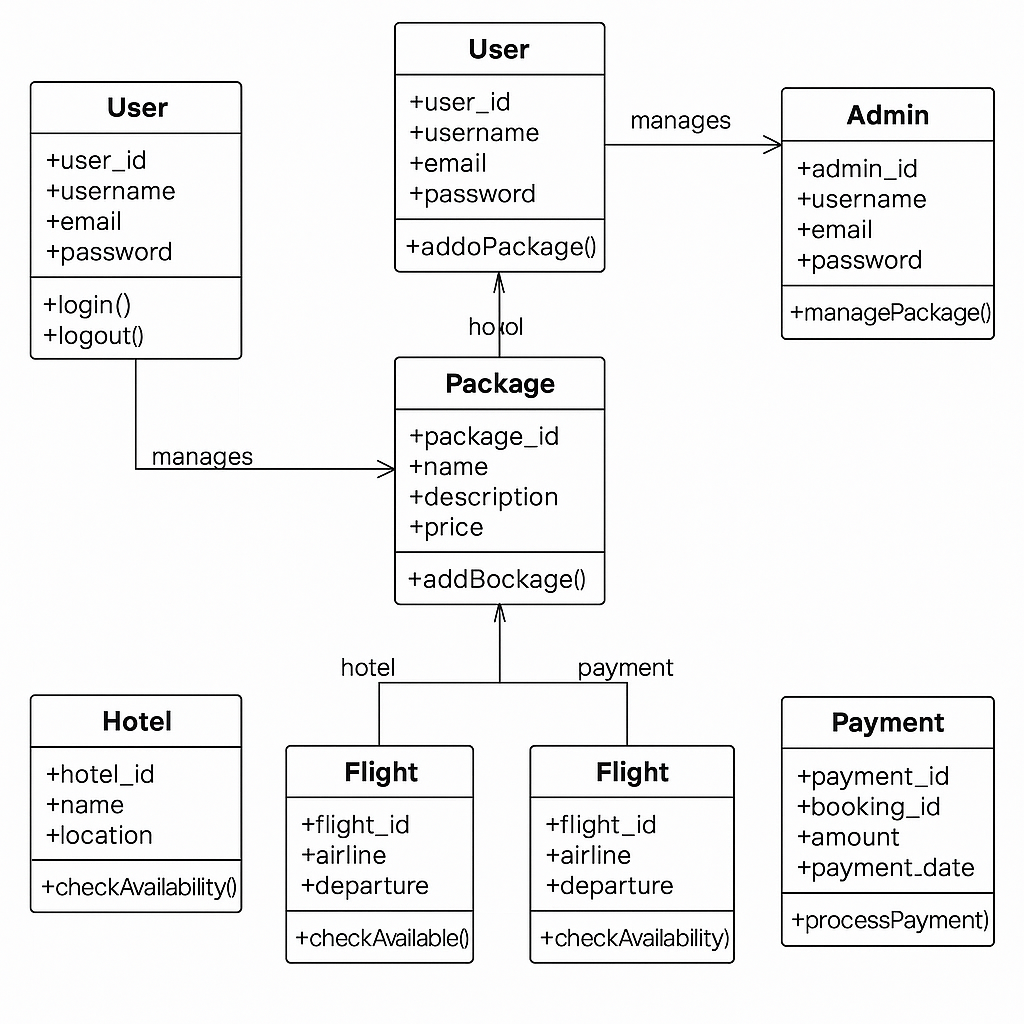
\includegraphics[width=1.0\textwidth]{./figures/UML Diagram/uml2.0.png} % Replace with your actual UML diagram path
\captionof{figure}{UML Diagram}
\end{center}
\vspace{0.5cm}

\subsection{Activity Diagram}
\subsubsection{Description}
An Activity Diagram models the flow of control in a system, representing the sequence of activities and their transitions. It visually represents workflows such as business processes or the flow of an algorithm, using actions, decisions, start and end points, and parallel processing.

\subsubsection{Usage}
\begin{itemize}
    \item \textbf{Workflow Representation:} Used to model high-level business processes or system workflows.
    \item \textbf{Decision Making:} Helps in visualizing conditional logic, showing decision points and alternative flows.
    \item \textbf{Parallel Processes:} Represents parallel processing or branching in a system.
\end{itemize}

\subsubsection{Key Elements}
\begin{itemize}
    \item \textbf{Initial Node:} Marks the starting point of the process.
    \item \textbf{Activity/Action:} Represents tasks or operations performed.
    \item \textbf{Decision Node:} Represents branching in the workflow, where a choice must be made.
    \item \textbf{Merge Node:} Combines multiple flows back into a single flow after decision points.
    \item \textbf{Final Node:} Marks the end of the process.
\end{itemize}

\vspace{0.5cm}
\begin{center}
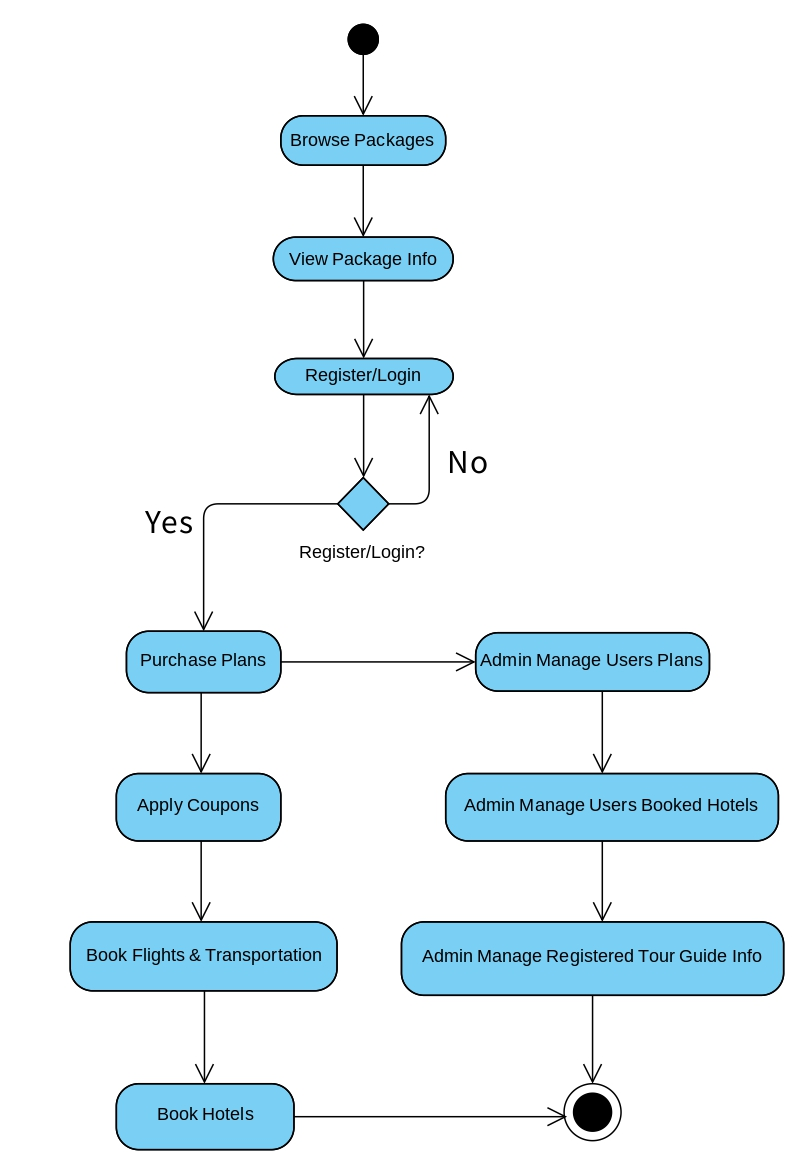
\includegraphics[width=1.0\textwidth]{./figures/Activity Diagram/actd.jpg} % Replace with your actual Activity Diagram path
\captionof{figure}{Activity Diagram for Odyssey Travel Agency Software}
\end{center}
\vspace{0.5cm}


\vspace{0.5cm}
\begin{center}
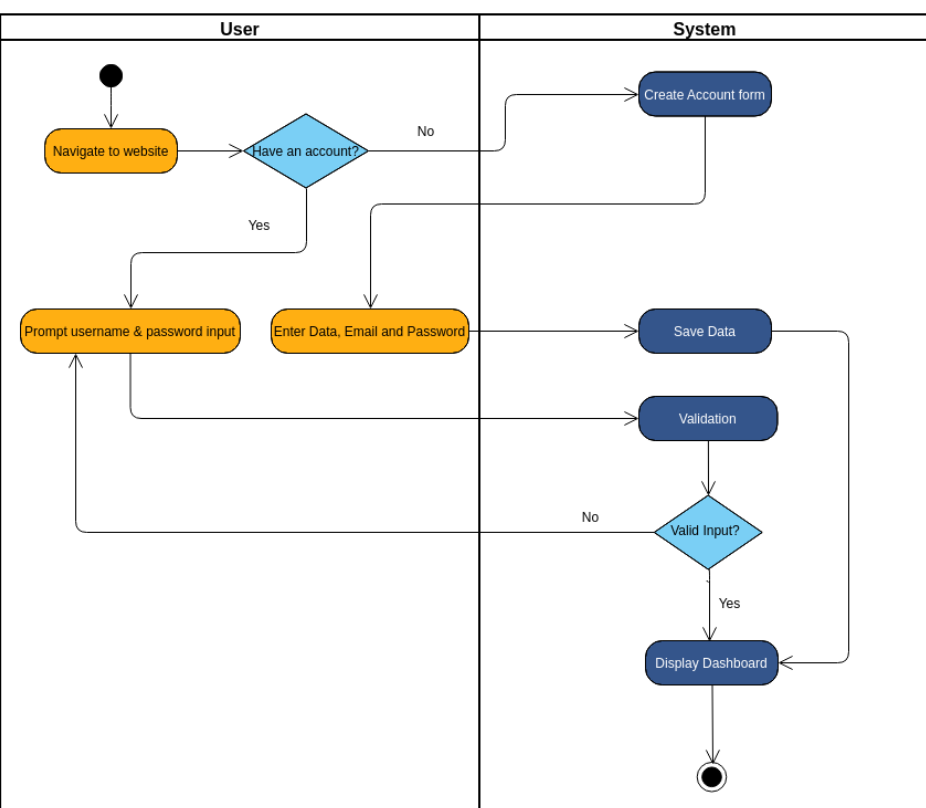
\includegraphics[width=0.8\textwidth]{./figures/Activity Diagram/1_reg.png} % Replace with your actual Activity Diagram path
\captionof{figure}{Activity Diagram Of Login and Registra   tion System} 
\end{center}
\vspace{0.5cm}

\vspace{0.5cm}
\begin{center}
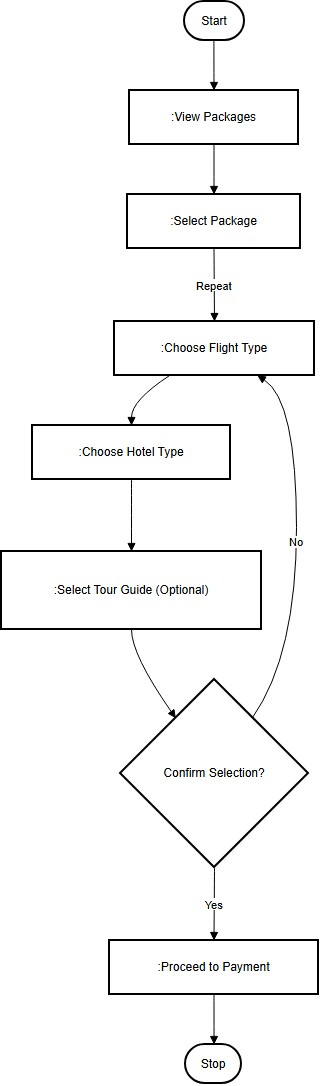
\includegraphics[width=0.5\textwidth]{./figures/Activity Diagram/2_activity.jpg} % Replace with your actual Activity Diagram path
\captionof{figure}{Package Selection Activity Diagram}
\end{center}
\vspace{0.5cm}

\vspace{0.5cm}
\begin{center}
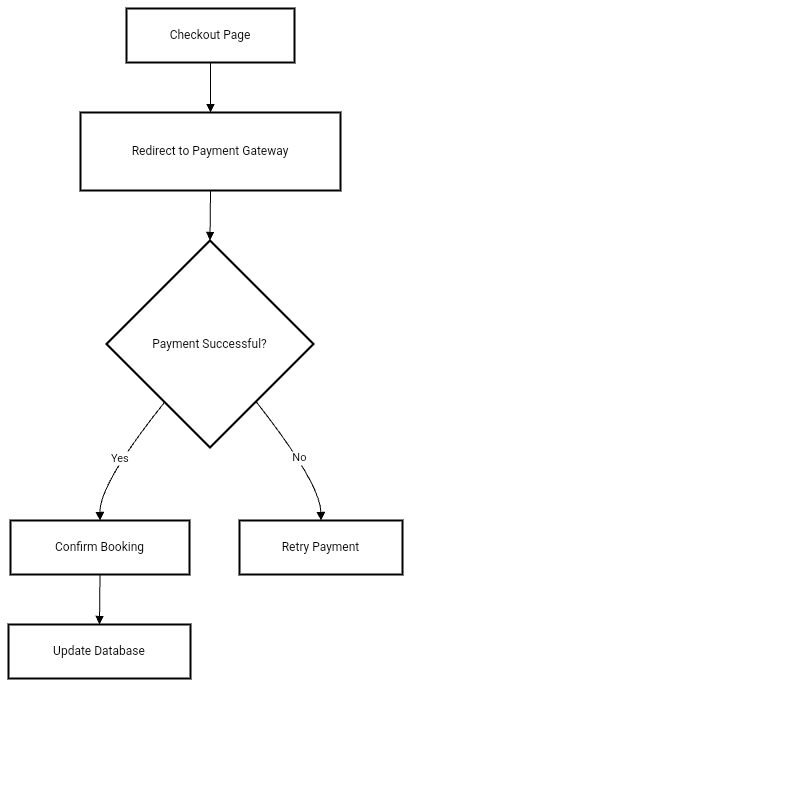
\includegraphics[width=0.8\textwidth]{./figures/Activity Diagram/3_acivity.png} % Replace with your actual Activity Diagram path
\captionof{figure}{Payment System Activity Diagram}
\end{center}
\vspace{0.5cm}

\vspace{0.5cm}
\begin{center}
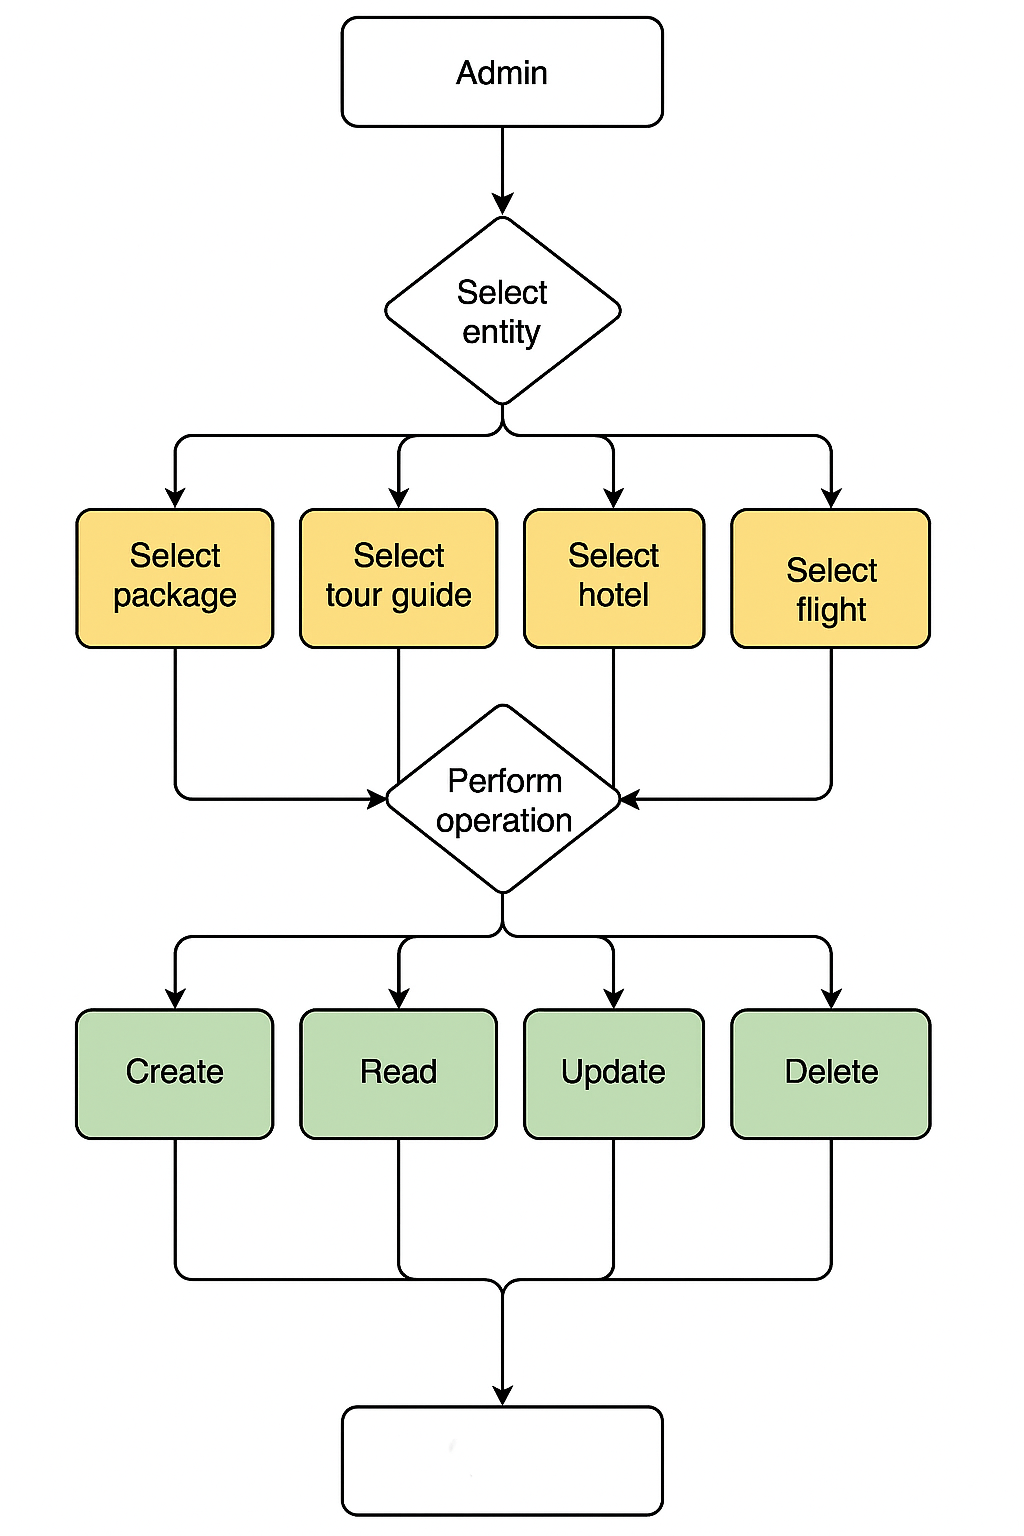
\includegraphics[width=0.8\textwidth]{./figures/Activity Diagram/4_crud_activity.png} % Replace with your actual Activity Diagram path
\captionof{figure}{Admin CRUD Operation Activity Diagram}
\end{center}
\vspace{0.5cm}


\subsection{Sequence Diagram}
\subsubsection{Description}
A Sequence Diagram focuses on the interaction between objects or components in a system over time. It shows the sequence of messages exchanged between objects to achieve a specific goal or functionality. It highlights the order of interactions and the roles of different components in a system.

\subsubsection{Usage}
\begin{itemize}
    \item \textbf{Object Interaction:} Helps in understanding the detailed interactions between different objects in a system.
    \item \textbf{Method Call Flow:} Useful for describing the flow of control during method calls and responses.
    \item \textbf{Debugging \& Testing:} Provides insight into the communication between objects, useful for debugging and designing test cases.
\end{itemize}

\subsubsection{Key Elements}
\begin{itemize}
    \item \textbf{Objects/Actors:} Represent entities that participate in the interaction.
    \item \textbf{Lifeline:} A dashed line that represents the lifespan of an object during the interaction.
    \item \textbf{Message Arrows:} Represent the messages sent between objects, showing the direction and order.
    \item \textbf{Activation Bar:} Indicates when an object is active (processing).
    \item \textbf{Return Message:} Represents the return of control from a method.
\end{itemize}

\vspace{0.5cm}
\begin{center}
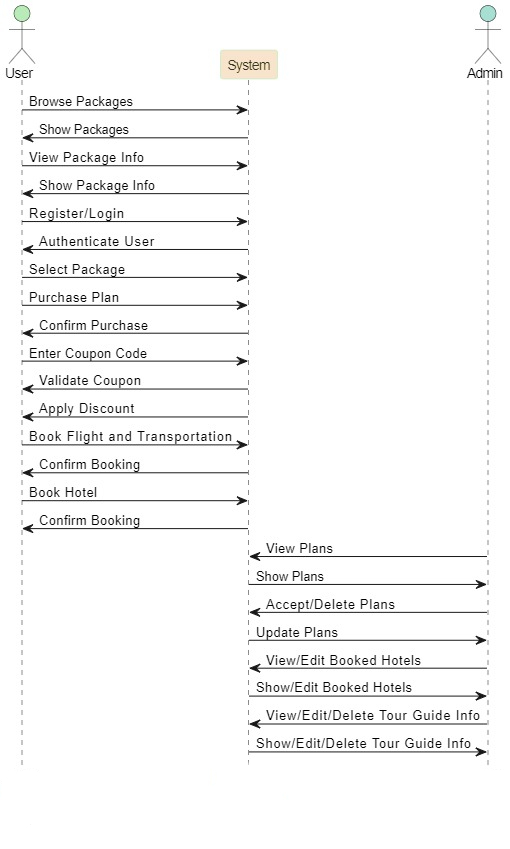
\includegraphics[width=0.8\textwidth]{./figures/Sequence Diagram/sqd.jpg} % Replace with your actual Sequence Diagram path
\captionof{figure}{Sequence Diagram of Odyssey Travel Agency Software}
\end{center}
\vspace{0.5cm}

\vspace{0.5cm}
\begin{center}
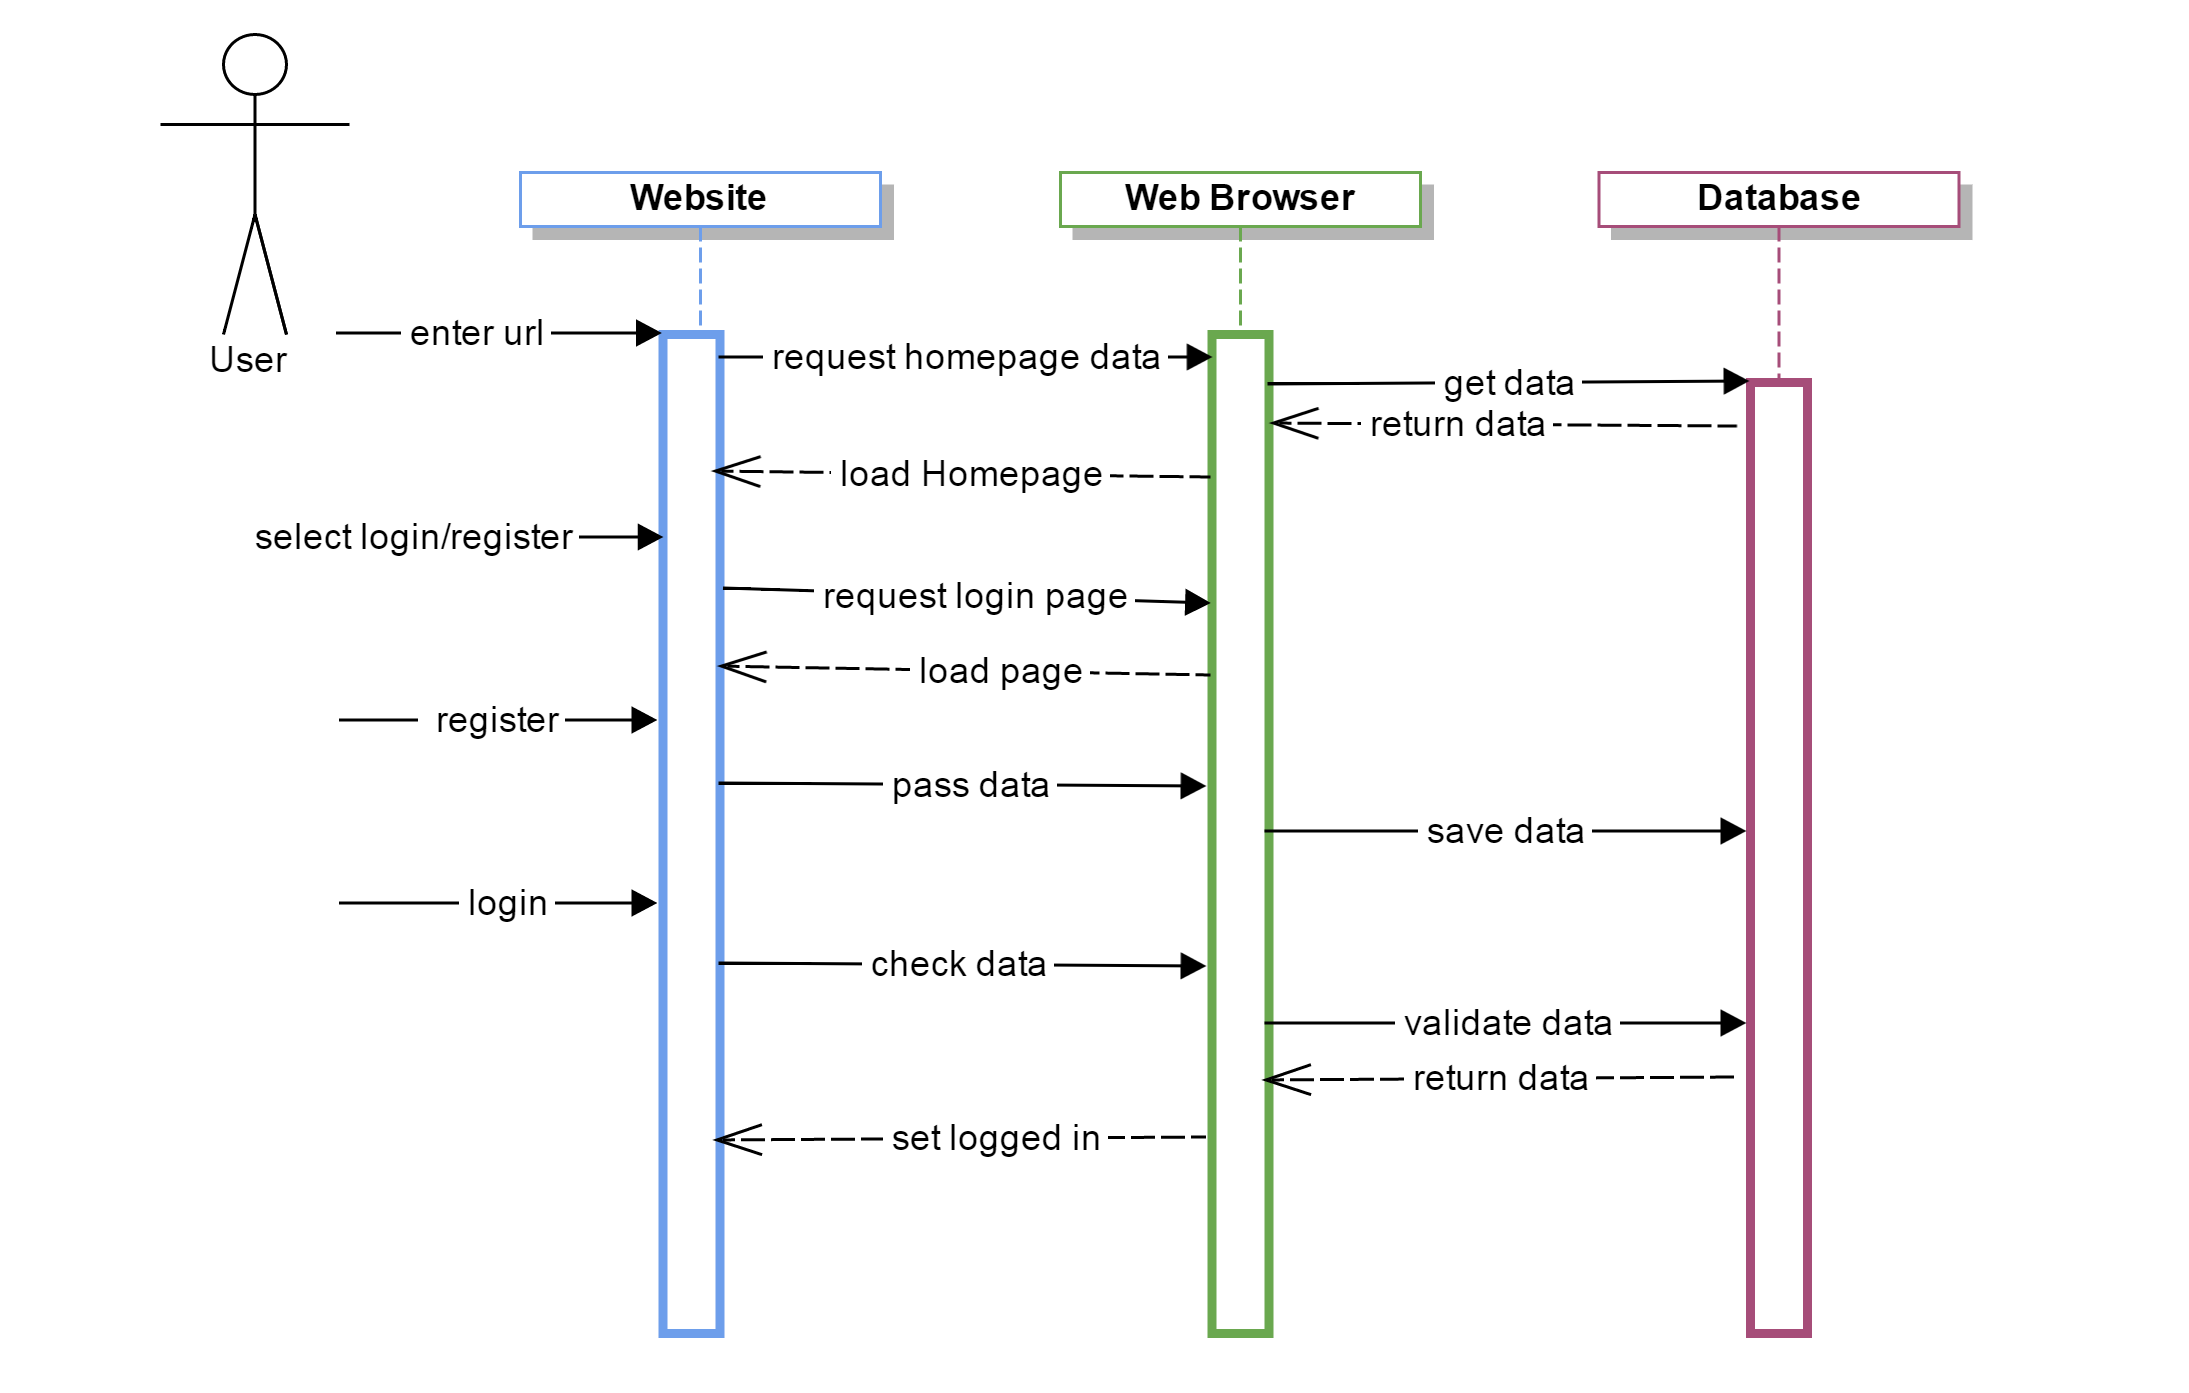
\includegraphics[width=0.9\textwidth]{./figures/Sequence Diagram/1_seq.png} % Replace with your actual Activity Diagram path
\captionof{figure}{Sequence Diagram Of Login and Registra   tion System} 
\end{center}
\vspace{0.5cm}

\vspace{0.5cm}
\begin{center}
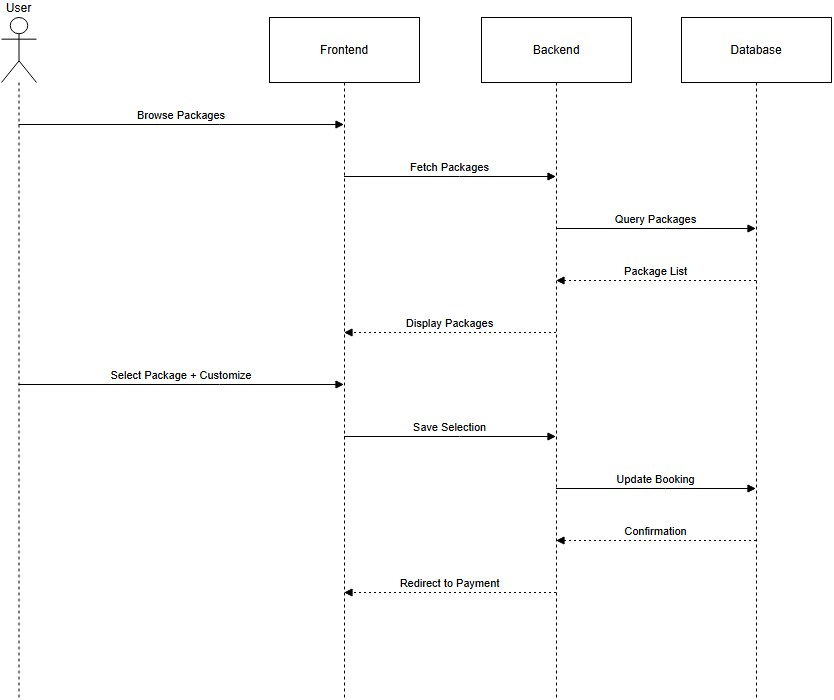
\includegraphics[width=1.0\textwidth]{./figures/Sequence Diagram/2_seq.jpg} % Replace with your actual Activity Diagram path
\captionof{figure}{Package Selection Sequence Diagram}
\end{center}
\vspace{0.5cm}

\vspace{0.5cm}
\begin{center}
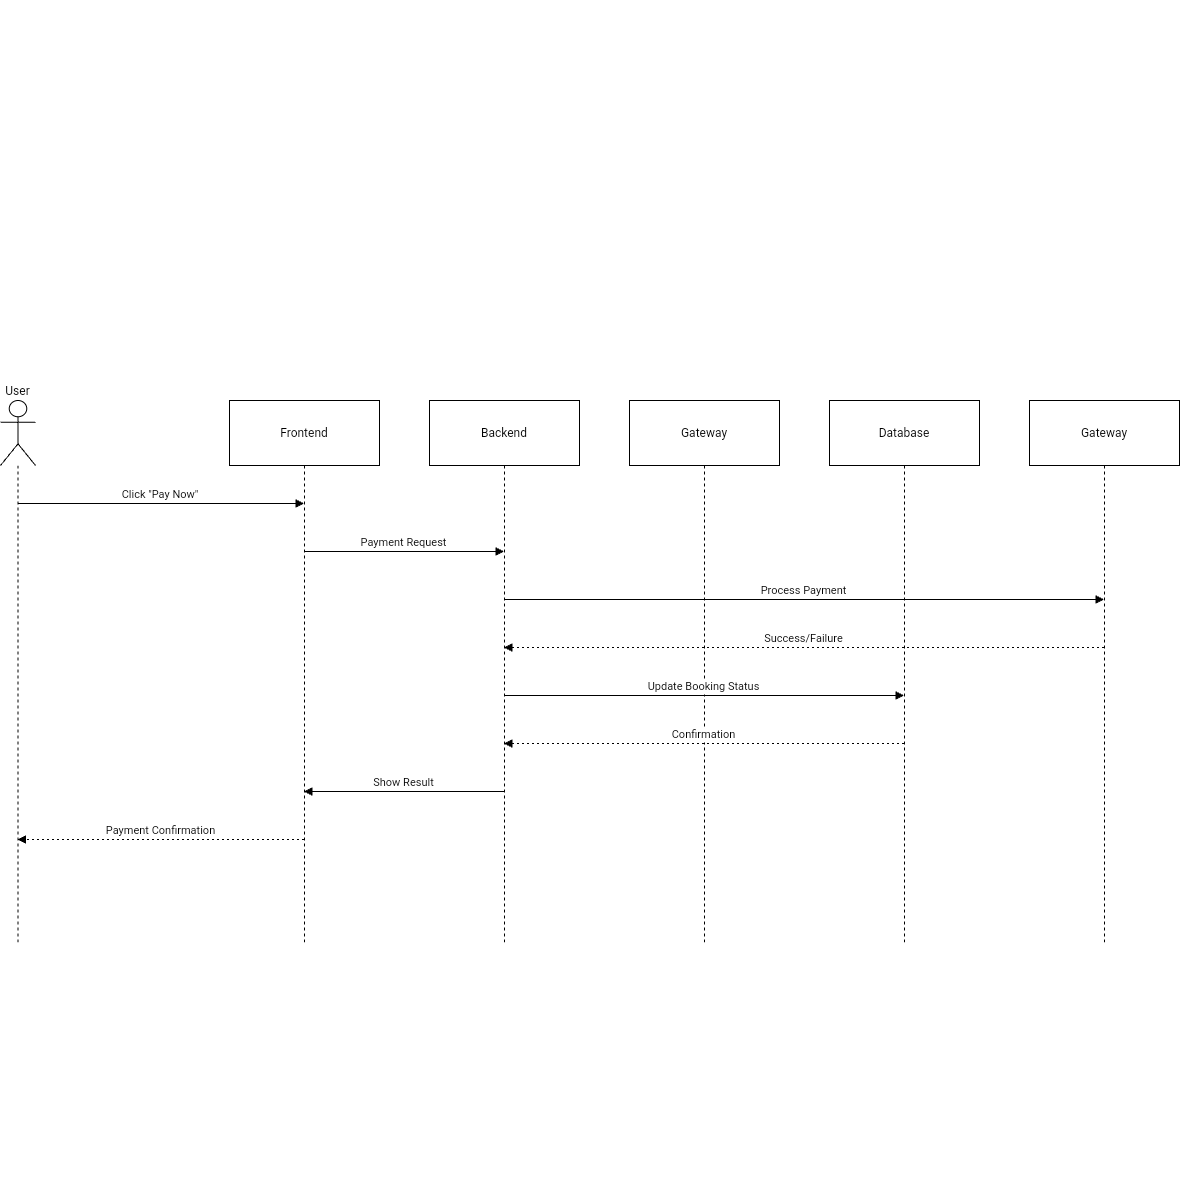
\includegraphics[width=1.0\textwidth]{./figures/Sequence Diagram/3_seq.png} % Replace with your actual Activity Diagram path
\captionof{figure}{Payment System Sequence Diagram}
\end{center}
\vspace{0.5cm}

\vspace{0.5cm}
\begin{center}
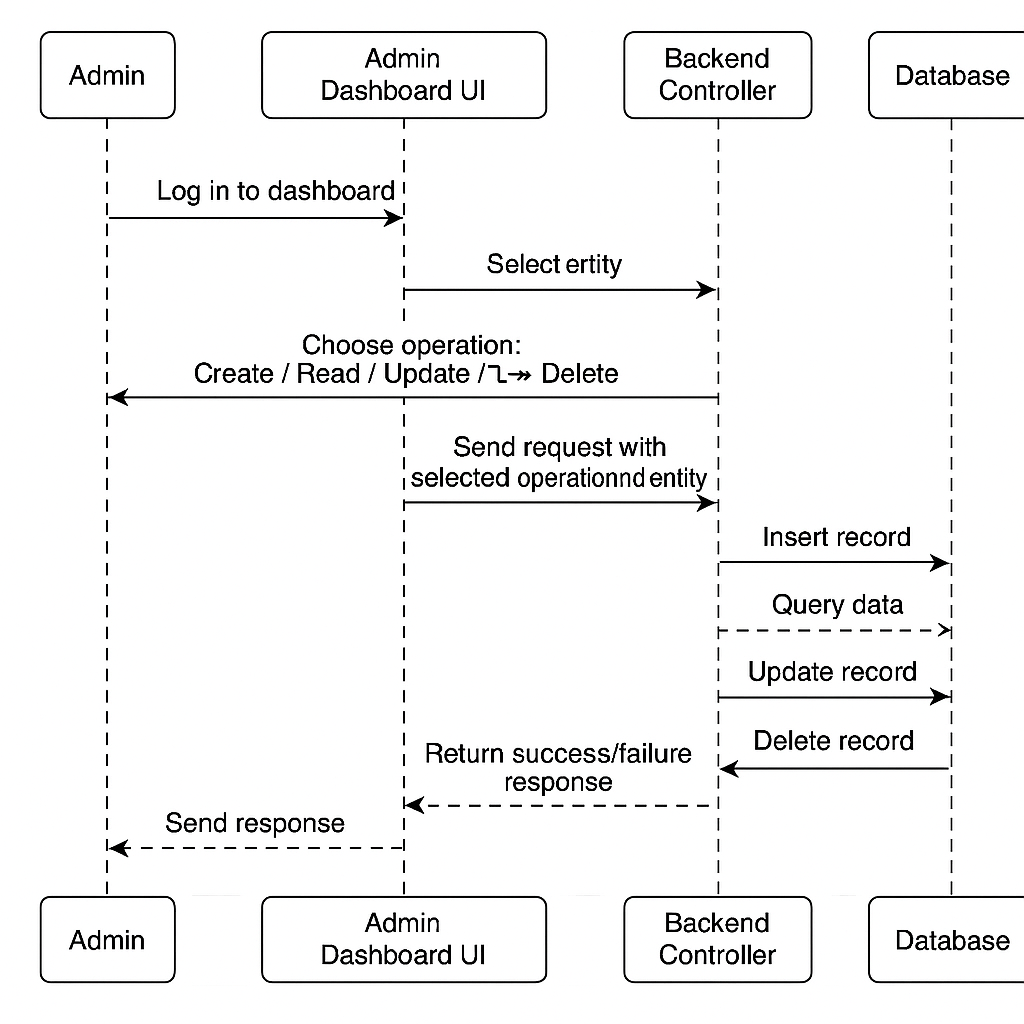
\includegraphics[width=0.8\textwidth]{./figures/Sequence Diagram/4_crud_sequence.png} % Replace with your actual Activity Diagram path
\captionof{figure}{Admin CRUD Operation Sequence Diagram}
\end{center}
\vspace{0.5cm}

\subsection{Use Case Diagram}
\subsubsection{Description}
A Use Case Diagram represents the functional requirements of a system by showing interactions between users (actors) and the system itself. It highlights the different use cases (functions or processes) the system performs and which actors are involved in each use case.

\subsubsection{Usage}
\begin{itemize}
    \item \textbf{Requirement Gathering:} Used to capture and clarify system functionality from the user's perspective.
    \item \textbf{System Scope:} Defines the boundaries of the system and what will be included in its functionality.
    \item \textbf{User Interaction:} Visualizes user-system interactions to understand how different users (actors) use the system.
\end{itemize}

\subsubsection{Key Elements}
\begin{itemize}
    \item \textbf{Actors:} Represent users or other systems that interact with the system.
    \item \textbf{Use Cases:} Represent functions or actions that the system performs (e.g., "Login," "Add Package").
    \item \textbf{System Boundary:} Represents the scope of the system and distinguishes between internal functions and external actors.
    \item \textbf{Associations:} Arrows or lines connecting actors to use cases, indicating their involvement.
\end{itemize}

\vspace{0.5cm}
\begin{center}
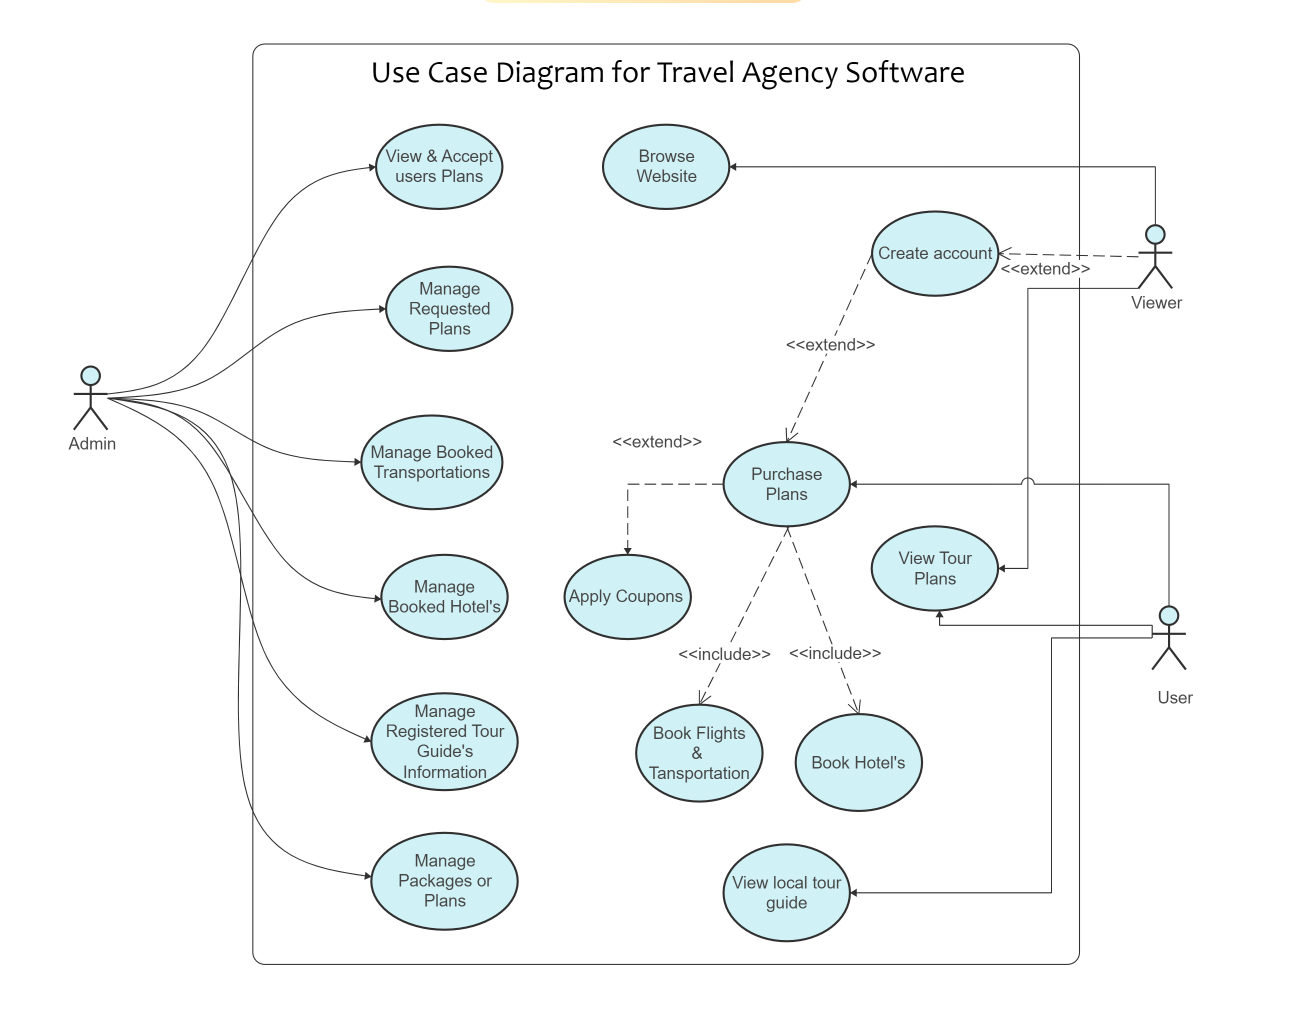
\includegraphics[width=0.8\textwidth]{./figures/Use Case Diagrams/uc_1.3.png} % Replace with your actual Use Case Diagram path
\captionof{figure}{Use Case Diagram for Odyssey Travel Agency Software}
\end{center}
\vspace{0.5cm}

\vspace{0.5cm}
\begin{center}
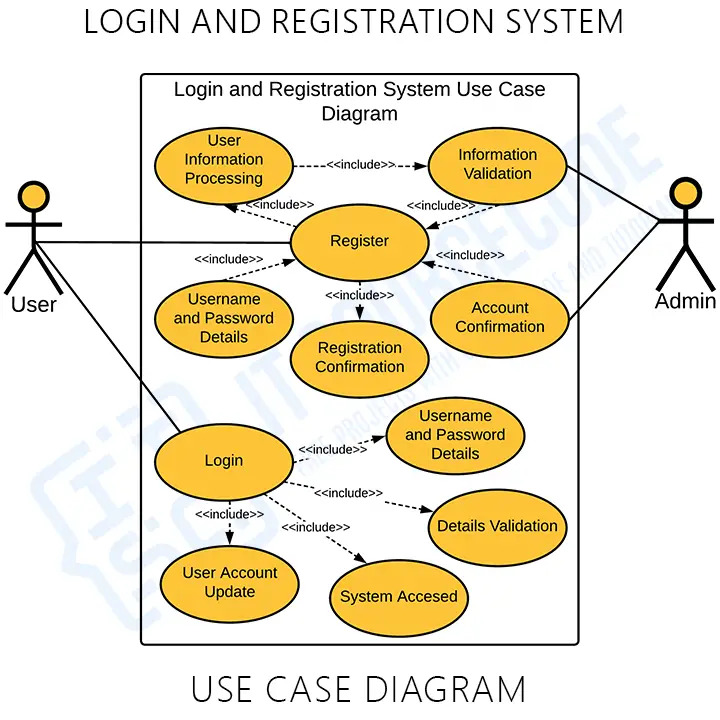
\includegraphics[width=0.8\textwidth]{./figures/Use Case Diagrams/1_usecase.jpg} % Replace with your actual Activity Diagram path
\captionof{figure}{Use Case Diagram Of Login and Registra   tion System} 
\end{center}
\vspace{0.5cm}

\vspace{0.5cm}
\begin{center}
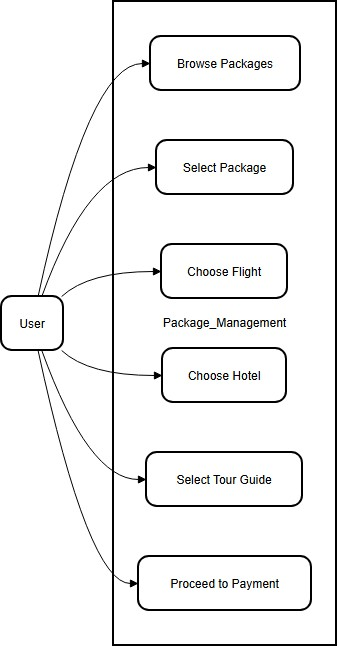
\includegraphics[width=0.5\textwidth]{./figures/Use Case Diagrams/2_usecaase.jpg} % Replace with your actual Activity Diagram path
\captionof{figure}{Package Selection Use Case Diagram}
\end{center}
\vspace{0.5cm}

\vspace{0.5cm}
\begin{center}
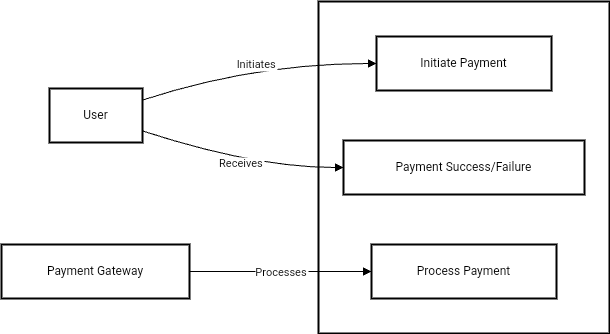
\includegraphics[width=0.8\textwidth]{./figures/Use Case Diagrams/3_usecase.png} % Replace with your actual Activity Diagram path
\captionof{figure}{Payment System Use Case Diagram}
\end{center}
\vspace{0.5cm}

\vspace{0.5cm}
\begin{center}
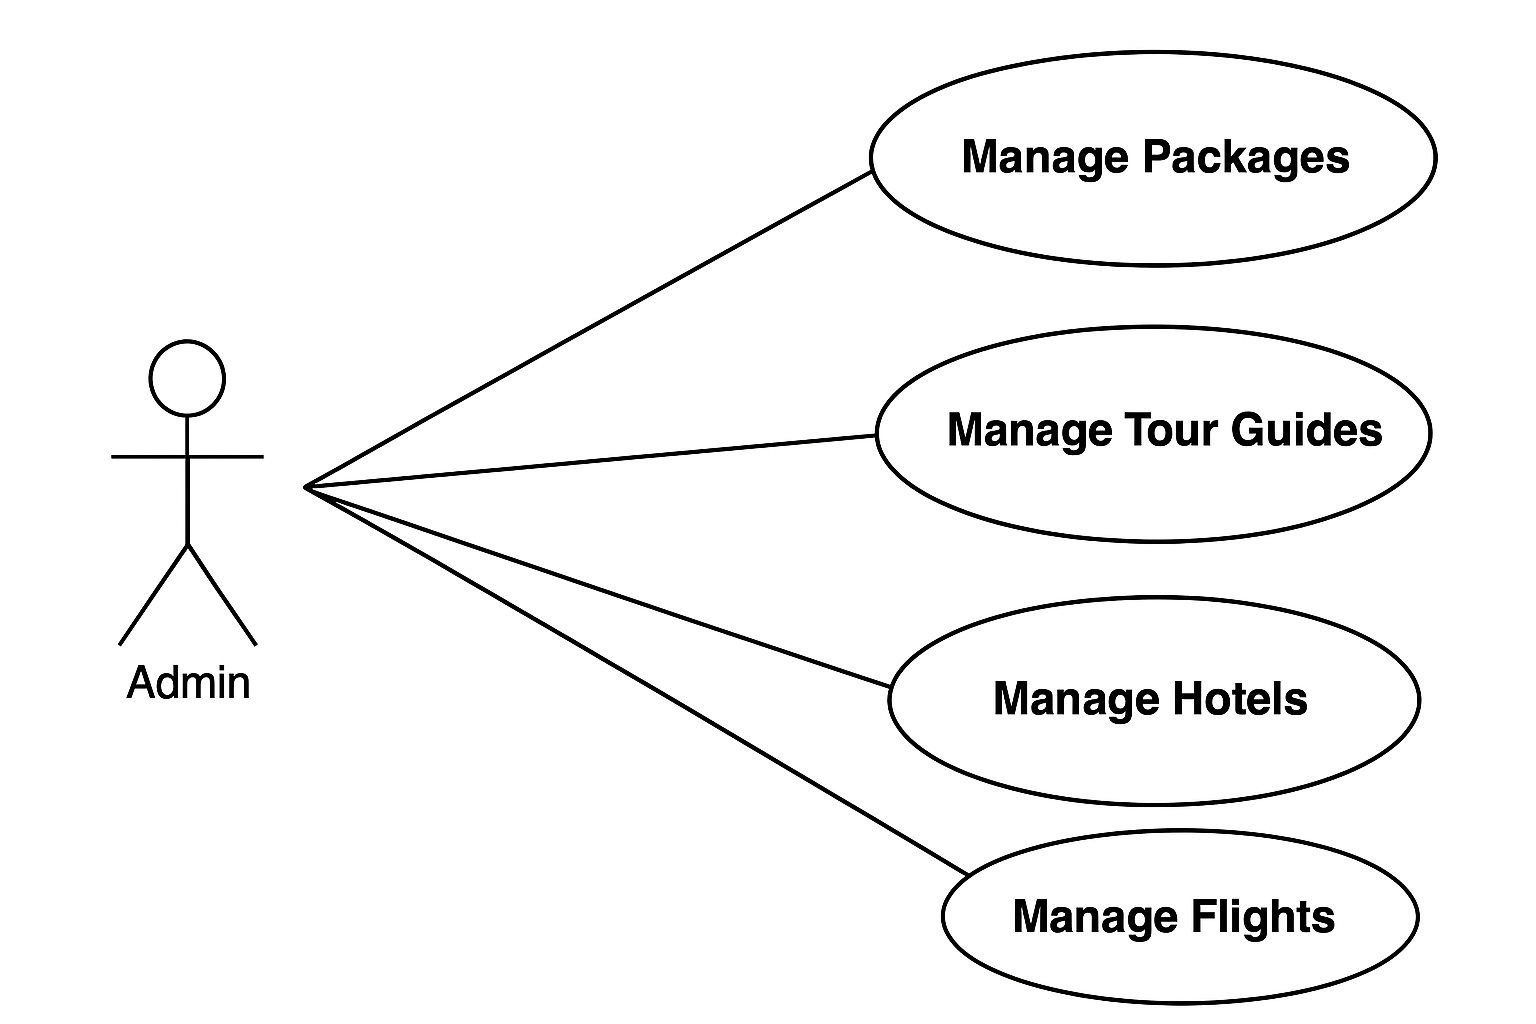
\includegraphics[width=0.8\textwidth]{./figures/Use Case Diagrams/4_crud_usecase.png} % Replace with your actual Activity Diagram path
\captionof{figure}{Admin CRUD Operation Use Case Diagram}
\end{center}
\vspace{0.5cm}
\section{ER Diagram}
\vspace{0.5cm}
\begin{center}
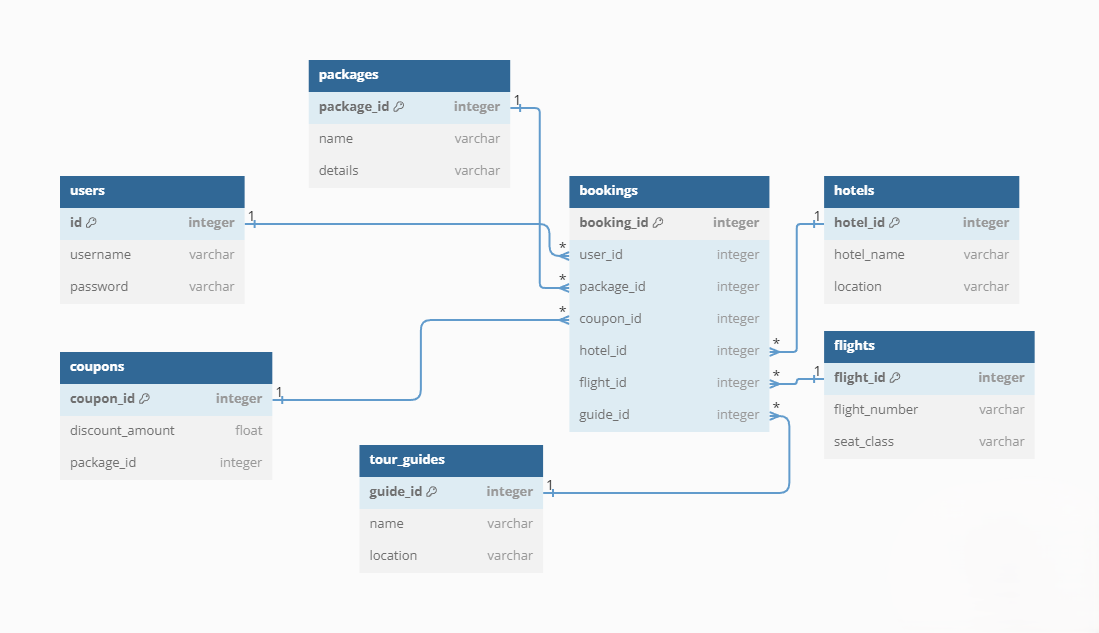
\includegraphics[width=1.0\textwidth]{./figures/ER Diagram/erd.png} % Replace with your actual Activity Diagram path
\captionof{figure}{ER Diagram for Odyssey Travel Agency Software}
\end{center}
